% fig_ejer1a_sum.tex — Componentes de x1(t) = 2u(t) + u(t-1) - 3u(t-4)
\documentclass[tikz]{standalone}
\usepackage{pgfplots}
\usepgfplotslibrary{groupplots}
\pgfplotsset{compat=1.18}
\definecolor{utnblue}{RGB}{0,102,204}
\definecolor{utnred}{RGB}{204,0,0}
\definecolor{utngreen}{RGB}{0,153,76}

\begin{document}
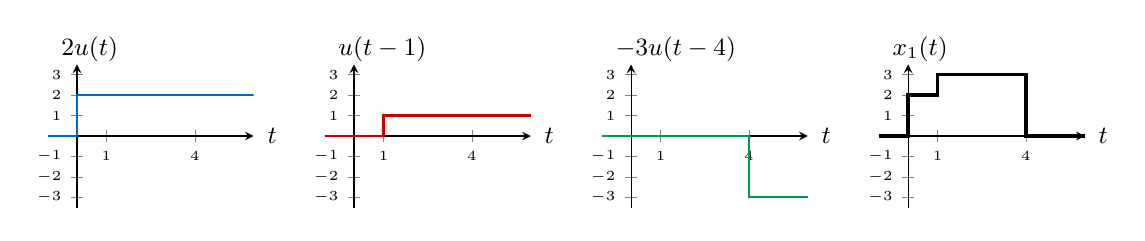
\begin{tikzpicture}
    \begin{groupplot}[
        group style={group size=4 by 1, horizontal sep=0.9cm},
        width=4.2cm, height=3.4cm,
        axis lines=middle,
        xmin=-1, xmax=6, ymin=-3.5, ymax=3.5,
        xtick={0,1,4}, ytick={-3,-2,-1,0,1,2,3},
        xticklabel style={font=\tiny}, yticklabel style={font=\tiny},
        every axis plot/.append style={thick},
        every axis x label/.append style={at={(ticklabel* cs:1.02)}, anchor=west, font=\small},
        every axis y label/.append style={at={(rel axis cs:0.02,0.95)}, anchor=south west, font=\small},
    ]
    % Componente 1: 2u(t)
    \nextgroupplot[ylabel={$2u(t)$}, xlabel={$t$}]
    \addplot[utnblue] coordinates {(-1,0)(0,0)(0,2)(6,2)};

    % Componente 2: u(t-1)
    \nextgroupplot[ylabel={$u(t-1)$}, xlabel={$t$}]
    \addplot[utnred] coordinates {(-1,0)(1,0)(1,1)(6,1)};

    % Componente 3: -3u(t-4)
    \nextgroupplot[ylabel={$-3u(t-4)$}, xlabel={$t$}]
    \addplot[utngreen] coordinates {(-1,0)(4,0)(4,-3)(6,-3)};

    % Suma total
    \nextgroupplot[ylabel={$x_1(t)$}, xlabel={$t$}]
    \addplot[black, very thick] coordinates {(-1,0)(0,0)(0,2)(1,2)(1,3)(4,3)(4,0)(6,0)};
    \end{groupplot}
\end{tikzpicture}
\end{document}
